\documentclass[a4paper, fleqn]{article}

\usepackage{amsmath}
\usepackage{enumitem}
\usepackage{graphicx}
\usepackage[page]{appendix}
\usepackage{listings}

\begin{document}

\title{Lab Exercise VII \\ Making Maps I: Introduction to Spatial Analysis, Data Visualization and Map Design}
\author{Basil R. Yap}
\date{2018 February 19}
\maketitle

\section{Part I}

\begin{itemize}
\item \textbf{Description of functions: }\begin{itemize}
\item \textit{acled} : returns the entirety of the dataframe (or up to the print limit for rows and/or columns)
\item \textit{summary(acled)} : returns a summary of the data based on its respective columns
\item \textit{head(acled)} : returns the first few rows of the dataframe
\item \textit{tail(acled)} : returns the last few rows of the dataframe
\end{itemize}
\item \textbf{Number of events with more than 400 fatalities: }28
\item \textbf{Country with the largest number of events: }Egypt
\item \textbf{Description of functions: }\begin{itemize}
\item \textit{dmy()} : converts a string with format day-month-year into lubridate package's date data format
\item \textit{wday()} : returns a numerical value corresponding to the weekday component stored within lubridate package's date data format, where 1 corresponds to Monday and 7 to Sunday
\end{itemize}
\item \textbf{The day of the week where events occur most frequently: }Saturday
\end{itemize}
\pagebreak
\section{Part II}
\begin{itemize}
\item \textbf{Description of functions: }\begin{itemize}
\item \textit{substr()} : returns a sequential snippet of a string based on two positional arguments defining the start and end of the sequence
\item \textit{aggregate()} : returns values based on function on column where values are grouped by the distinct cases of another column
\end{itemize}
\item \textbf{Event type with the largest number of events: }Violence against civilians 
\item \textbf{Year with most fatalities: } 1999 \textit{[Figure 1]}
\begin{figure}[h!]
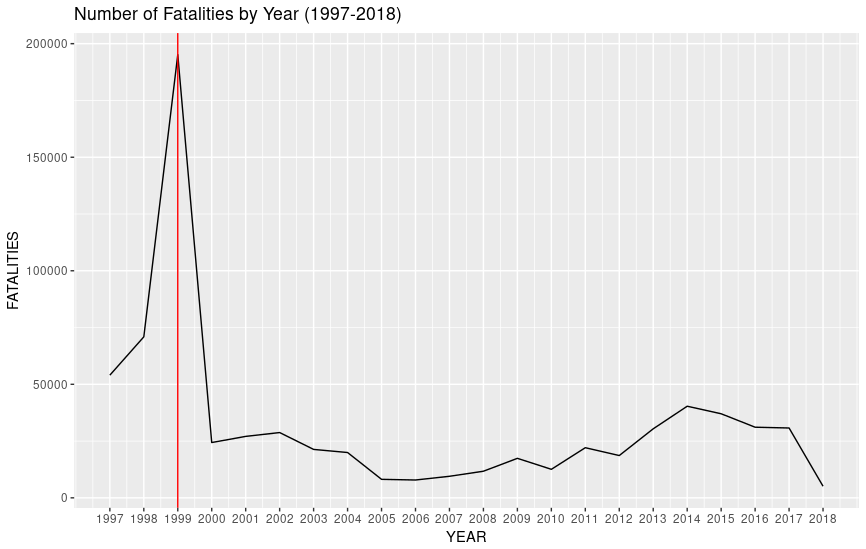
\includegraphics[width=\linewidth]{./assets/201803220315.png}
\label{figure:img1}
\end{figure}
\item \textit{[Figure 2]}\\\begin{figure}[h!]
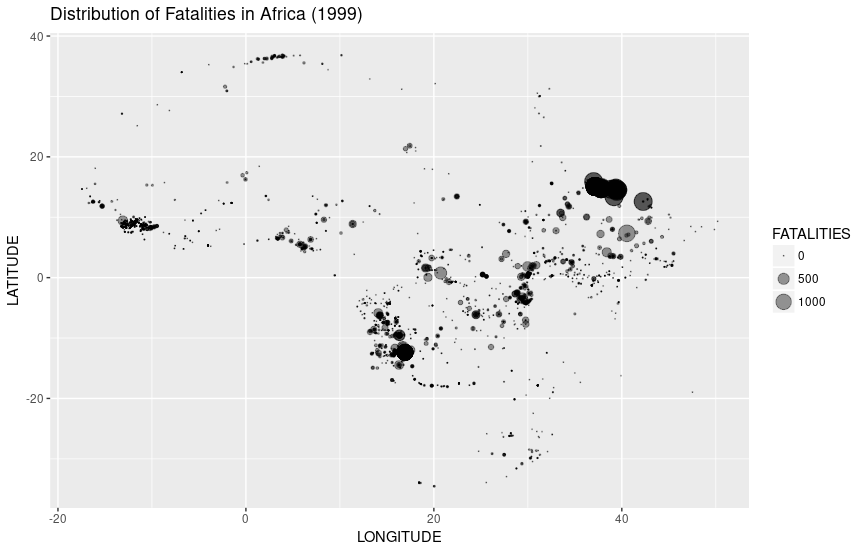
\includegraphics[width=\linewidth]{./assets/201803220342.png}
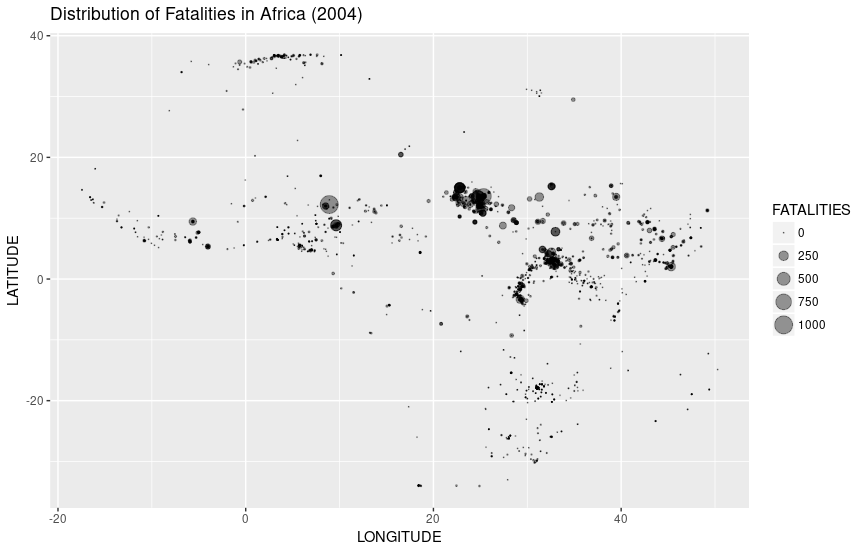
\includegraphics[width=\linewidth]{./assets/201803220344.png}
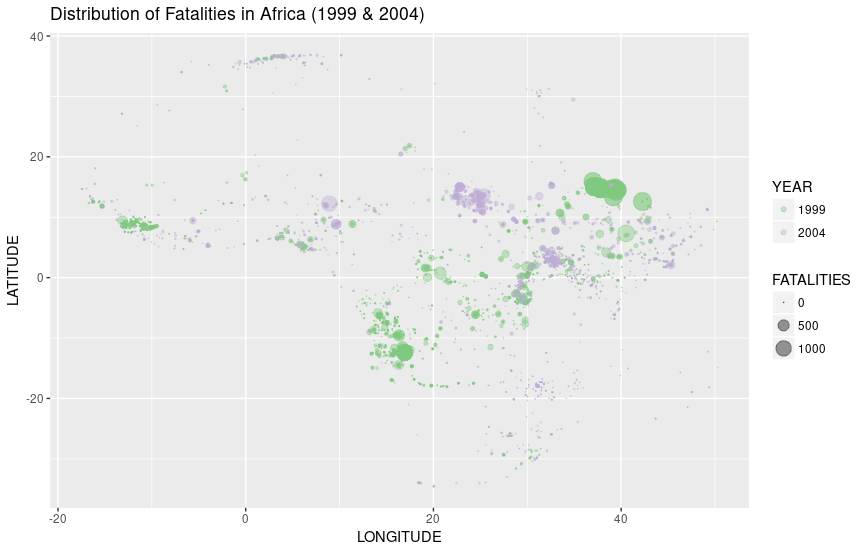
\includegraphics[width=\linewidth]{./assets/201803220355.png}
\end{figure}
\end{itemize}
\end{document}